\documentclass[10.5pt]{article}
\usepackage{graphicx}
\usepackage{amsmath, amsfonts, amssymb,amsthm}
\usepackage{centernot}
\usepackage[includeheadfoot,margin=0.5in]{geometry} % For page dimensions
\usepackage{fancyhdr}
\usepackage{enumerate} % For custom lists
\usepackage{tikz-cd}

\fancyhf{}
\lhead{Math 426hw4}
\rhead{Tighe McAsey - 37499480}
\pagestyle{fancy}

% Page dimensions
\geometry{a4paper}

\theoremstyle{definition}
\newtheorem{pb}{}
\usepackage{color}

% Commands:

\newcommand{\set}[1]{\{#1\}}
\newcommand{\abs}[1]{\lvert#1\rvert}
\newcommand{\norm}[1]{\lvert\lvert#1\rvert\rvert}
\newcommand{\gen}[1]{\langle #1 \rangle}
\newcommand{\tand}{\text{ and }}
\newcommand{\tor}{\text{ or }}
\newcommand{\ism}{\simeq}

\begin{document}
    \begin{pb}
        \textbf{Lemma.} Any integer matrix \(M\) of rank 2 can be reduced by row operations to a unique representative of the form
        \begin{align*}
            A = \begin{bmatrix} a & b \\ 0 & d \end{bmatrix} \quad 0 < a, d \tand 0 \leq b < d
        \end{align*}

        For existence, we show that we have elements of the above form in the span of \(\gen{we_1 + xe_2} \oplus \gen{ye_1 + ze_2}\). If \(w = 0\), then \(y \neq 0\) (if \(y < 0\) multiply \(ye_1 + ze_2\) by \(-1\), same for \(x < 0\) with \(xe_2\)), so by long division, there exists some \(m\) such that \(0 \leq z - mx < x\), so that the matrix in this case is
        \(\begin{bmatrix} y & z - mx \\ 0 & x \end{bmatrix}\)
        
        Now assuming that \(w \neq 0\), by Bezout's identity there exist integers \(p,q\) (\(p \neq 0\)) such that \(pw + qy = (w,y) = a\). Then we have \(ae_1 + re_2 \in \gen{we_1 + xe_2} \oplus \gen{ye_1 + ze_2}\) for some \(r\). Subtracting since \(a \vert y\), we may subtract \(y/a(ae_1 + re_2)\) from \(ye_1 + ze_2\). This gives us the element \((z - ry/a)e_2\), which is non-zero since \(ae_1 + re_2 \not \in \gen{ye_1 + ze_2}\) since we had \(p \neq 0\). Rewrite \(d = \abs{z - ry/a}\), then once again by long division, we get some \(m\), such that \(0 \leq r - md < d\), subtracting \(md e_2\) from \(ae_1 + re_2\), and rewriting \(b = r-md\) gives us our desired rowspace representative \(\begin{bmatrix} a & b \\ 0 & d \end{bmatrix}\). We can see that in both cases \(w = 0\) and \(w \neq 0\) our constructed matrix has equal rowspace to the original, since we can construct it using only row swaps, adding and subtracting multiples of rows from eachother and multiplying the rows by \(\pm 1\).

        For uniqueness, we want to show that given \(0 < a,d,x,z\) and \(0 \leq y < z\) and \(0 \leq b < d\) we have
        \begin{align*}
            V := \gen{ae_1 + be_2}\oplus\gen{de_2} = U := \gen{xe_1 + ye_2}\oplus\gen{ze_2}
        \end{align*}
        exactly when \((a,b,d) = (x,y,z)\), equality of coefficients implying equality of modules is obvious so we prove the other direction. First assume that \(d e_2 \in U \iff z \vert d\), similarly \(z e_2 \in V \iff d \vert z\), so \(U = V\) implies that \(z = d\). Similarly, there exists some \(\ell \in \mathbb{Z}\) such that \(ae_1 + \ell e_2 \in U\) exactly when \(x \vert a\), and conversely there exists some \(k \in \mathbb{Z}\) such that \(xe_1 + ke_2 \in V\) exactly when \(a \vert x\), so that \(U = V\) implies that \(a = x\). Finally suppose that \(x = a \tand d = z\). Then \(ae_1 + be_2 \in U\) exactly when \(b \equiv y \mod d\), but since \(0 \leq b,y < d\), this means that \(U = V\) implies \(b = y\), this finishes the proof of uniqueness of representative.
        \newline

        \(G := \pi_1(S_1 \times S_1) \simeq \mathbb{Z} \times \mathbb{Z}\). Since \(G\) is abelian, in particular all of its subgroups are normal. We apply the correspondence of degree \(d\) covering spaces (up to isomorphism) with index \(d\) subgroups up to conjugacy of \(G \simeq \mathbb{Z} \times \mathbb{Z}\). Since each of the subgroups of \(G\) are normal, this reduces the problem to determining the number of subgroups \(H \subset G\) with \([G:H] = d\).

        We regard \(G\) as the free \(\mathbb{Z}\)-module, and write \(G = \gen{e_1} \oplus \gen{e_2}\), by the Structure Theorem for Finitely Generated Modules over a PID, a subgroup \(H \subset G\) has finite index if and only if \(H\) is free of rank 2, and furthermore if \(H = \gen{a e_1 + be_2} \oplus \gen{ce_1 + de_2}\), then we may take \(D = \text{Diag}(d_1,d_2)\) to be the smith normal form of
        \(\begin{bmatrix}a & b\\ c & d \end{bmatrix}\), where
        \begin{align*}
            [G:H] = d_2 = \det \begin{bmatrix}a & b\\ c & d \end{bmatrix}
        \end{align*}
        Now let \(H = \gen{a e_1 + be_2} \oplus \gen{ce_1 + de_2}\), \(K = \gen{we_1 + xe_2} \oplus \gen{ye_1 + ze_2}\), it is immedate that
        \begin{align*}
            H = K \iff \text{Rowsp}\begin{bmatrix}a & b\\ c & d \end{bmatrix} = \text{Rowsp}\begin{bmatrix}w & x\\ y & z \end{bmatrix}
        \end{align*}
        Finally reducing the problem to counting the number of integer matrices with determinant \(d\) up to equality of row spaces. Using the lemma, we can consider all integer matrices of the form
        \begin{align*}
            A = \begin{bmatrix} x & y \\ 0 & z \end{bmatrix} \quad 0 < x, z \tand 0 \leq y < z \tand \det A = xz = d
        \end{align*}
        Every matrix of this form with determinant \(d\) must have \(z \vert d\), so fixing \(0 < z \vert d\), there is a unique choice for \(x\), such that \(\det A = xz = d\), then each choice of \(0 \leq y < z\), we get a unique row space satisfying \(\det A = d\).
        counting these gives us the number of degree \(d\) covering spaces up to isomorphism is
        \begin{align*}
            \sum_{z \vert d} \# \set{0 \leq y < z \vert y \in \mathbb{Z}} = \sum_{k \vert d} k = \sigma(d)
        \end{align*}
        As desired.
    \end{pb}
    \newpage
    \begin{pb}
        \textbf{(a)} We consider the point \(x_0\) as the base point of the two loops. 
        Denote \(G := \pi_1(X,x_0)\). There are 3 degree 2 covering spaces of \(X\) up to isomorphism, with the same numbering convention as in the picture call these \((\tilde{X_1},p^1),(\tilde{X_2},p^2),(\tilde{X_3},p^3)\). To see this, note that groups of index 2 are normal, and invoke our correspondence between conjugacy classes of subgroups, so that we simply need to count the groups of index \(2\) in \(G = \gen{a}*\gen{b}\). In this case \(G/H \simeq C_2\) (since this is the only group of order 2) which is only possible when \(a^2 = 1, b^2 = 1\) and either \(a = b \neq 1\), or \(a = 1, b \neq 1\) or \(a \neq 1, b = 1\) in the quotient. The possible \(H\) giving these are
        \begin{align*}
            H_1 = N(\gen{a^2,ab^{-1}}) \quad H_2 = N(\gen{a^2,b}) \quad H_3 = N(\gen{b^2,a})
        \end{align*}
        So that there are at most 3 covering spaces of degree 2. 
        
        \begin{figure*}[h]
            \centering
            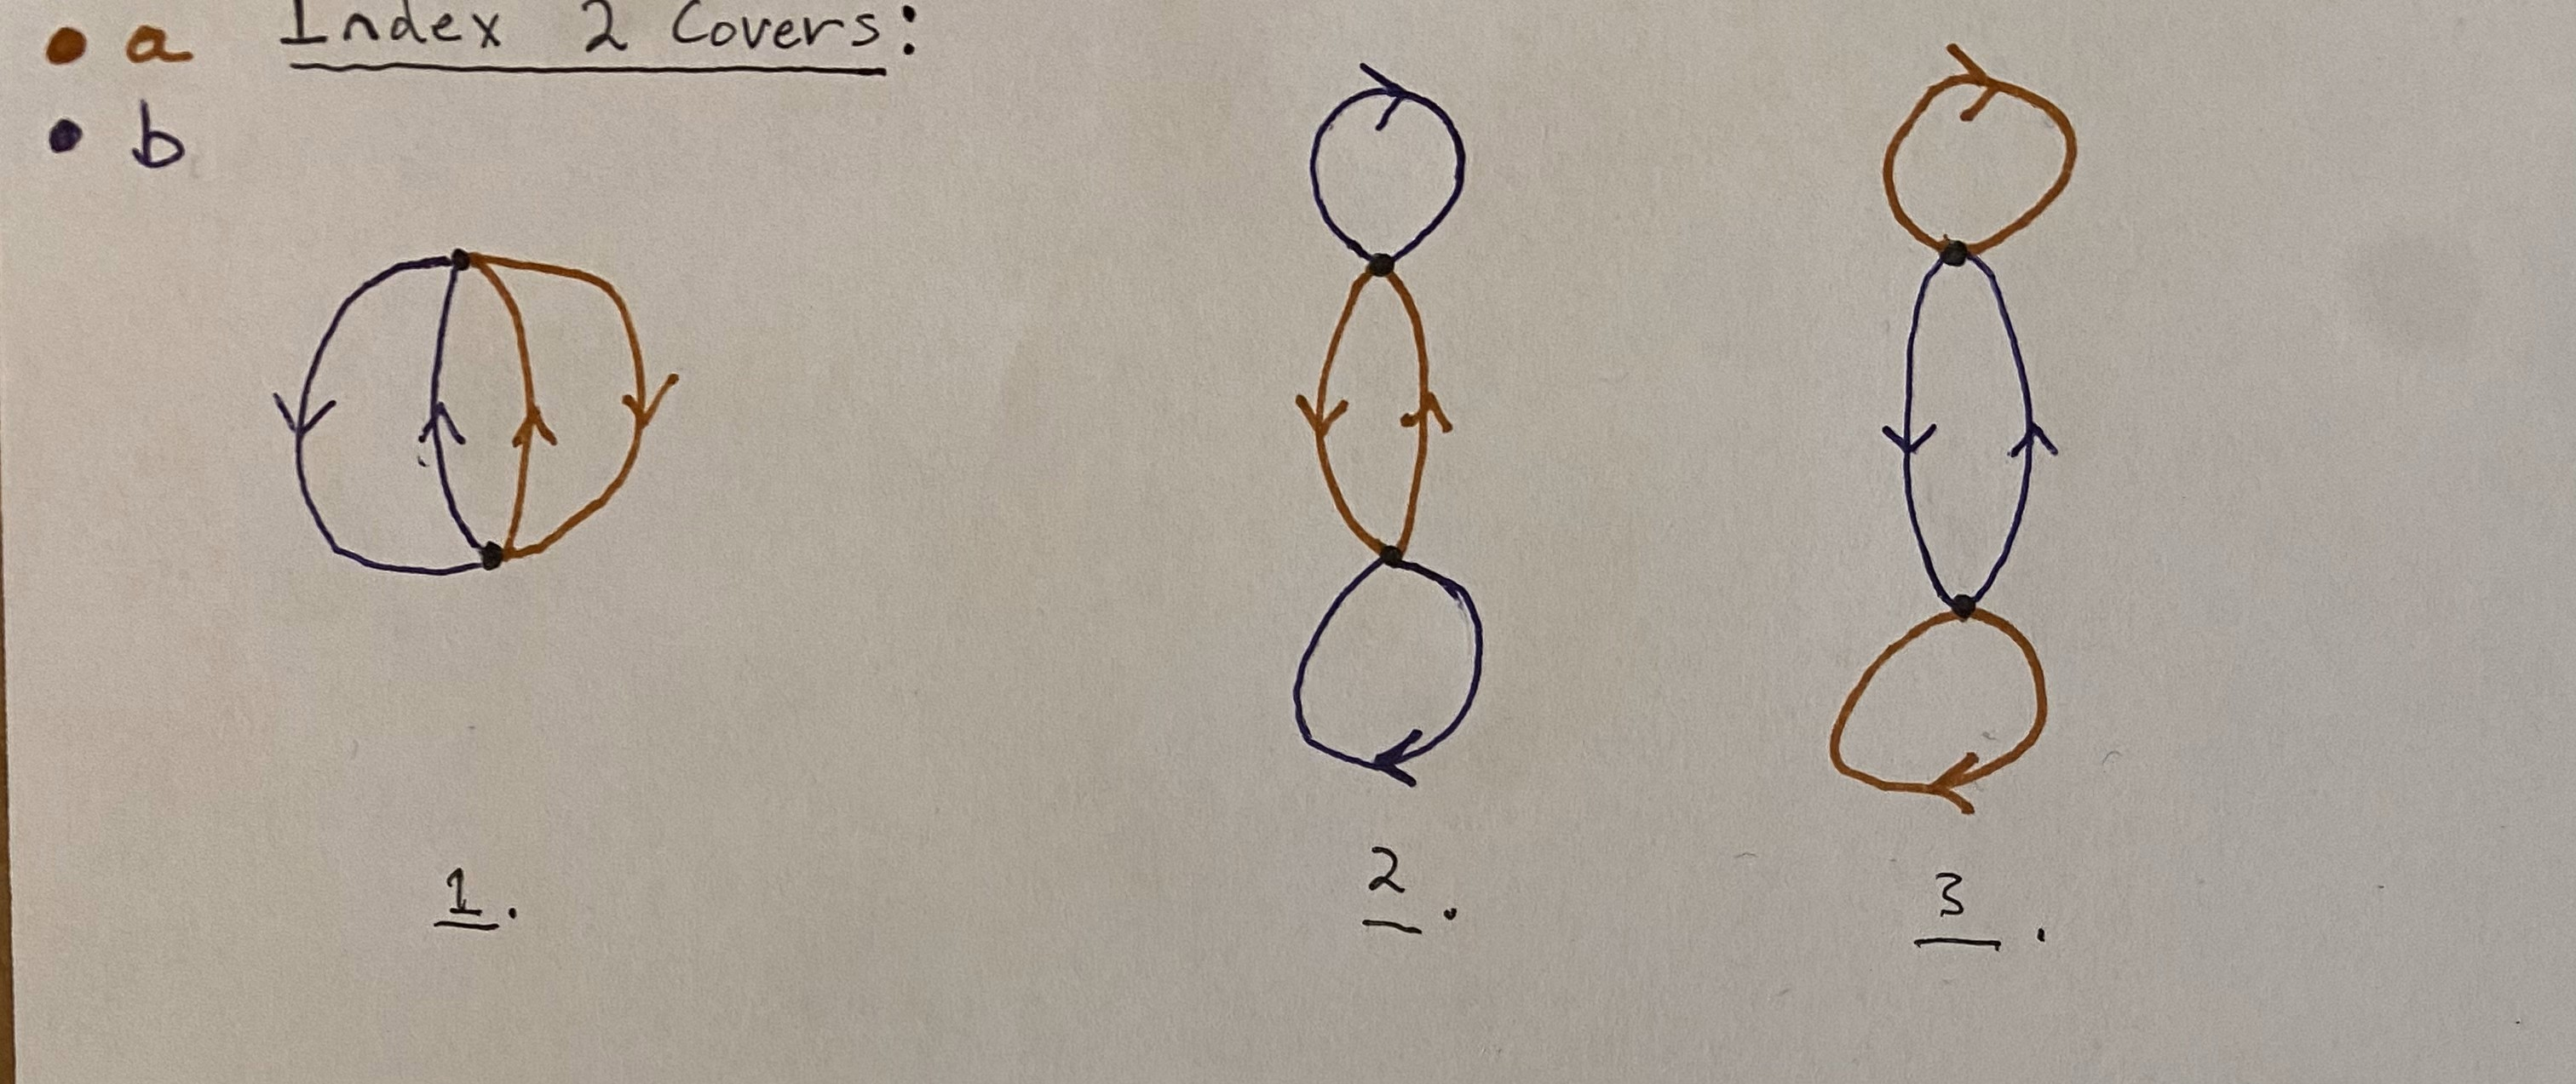
\includegraphics[width = \textwidth]{graphics/Degree 2 covers.jpg}
        \end{figure*}
        
        
        The three covering spaces drawn clearly fulfill the criteria to be covering spaces of \(X\) (they are path connected, locally path connected, Hausdorff and its clear each point has elementary neighborhoods). To see that these covering spaces are distinct, we note that any covering space transformation between them must send the lifts of \(x_0\) to lifts of \(x_0\). Now fix a lift \(\tilde{x}\) in covering space \(i\), and let \(\tilde{x_1}, \tilde{x_2}\) be the lifts of \(x_0\) in space \(j\), a necessary condition for a covering space morphism between spaces \(i\) and \(j\) is that
        \begin{align*}
            p^i_*\pi_1(\tilde{X_i},\tilde{x}) \subset p^j_*\pi_1(\tilde{X_j},\tilde{x_1}) \tor p^i_*\pi_1(\tilde{X_i},\tilde{x}) \subset p^j_*\pi_1(\tilde{X_j},\tilde{x_2})
        \end{align*}
        But then taking any lifts of \(x_0\), given by \(\tilde{x} \in \tilde{X_2}, \tilde{x}' \in \tilde{X_3}\) we have that \(b \in p^2_*\pi_1(\tilde{X_2},\tilde{x}) \tand a \in p^3_*\pi_1(\tilde{X_3},\tilde{x}')\), but
        \begin{align*}
            &a \not \in p^i_*\pi_1(\tilde{X_i},\tilde{y}), \; i \in \set{1,2} \; \tilde{y} \in F_{x_0} \\
            &b \not \in p^i_*\pi_1(\tilde{X_i},\tilde{y}), \; i \in \set{1,3} \; \tilde{y} \in F_{x_0}
        \end{align*}
        So in particular no such covering space isomorphisms may exist, so the three covering spaces drawn are all unique and are the degree 2 covering spaces of \(\tilde{X}\). As stated before index 2 subgroups are normal, so that in each of these cases \(N(H_i) = G\), implying that
        \begin{align*}
            \# N(H_i)/H_i = [G:H] = 2 \implies A(\tilde{X_i}) = C_2
        \end{align*}
        \newpage

        \textbf{(b)} There are 7 covering spaces, all included in the picture.

        \begin{figure*}[h]
            \centering
            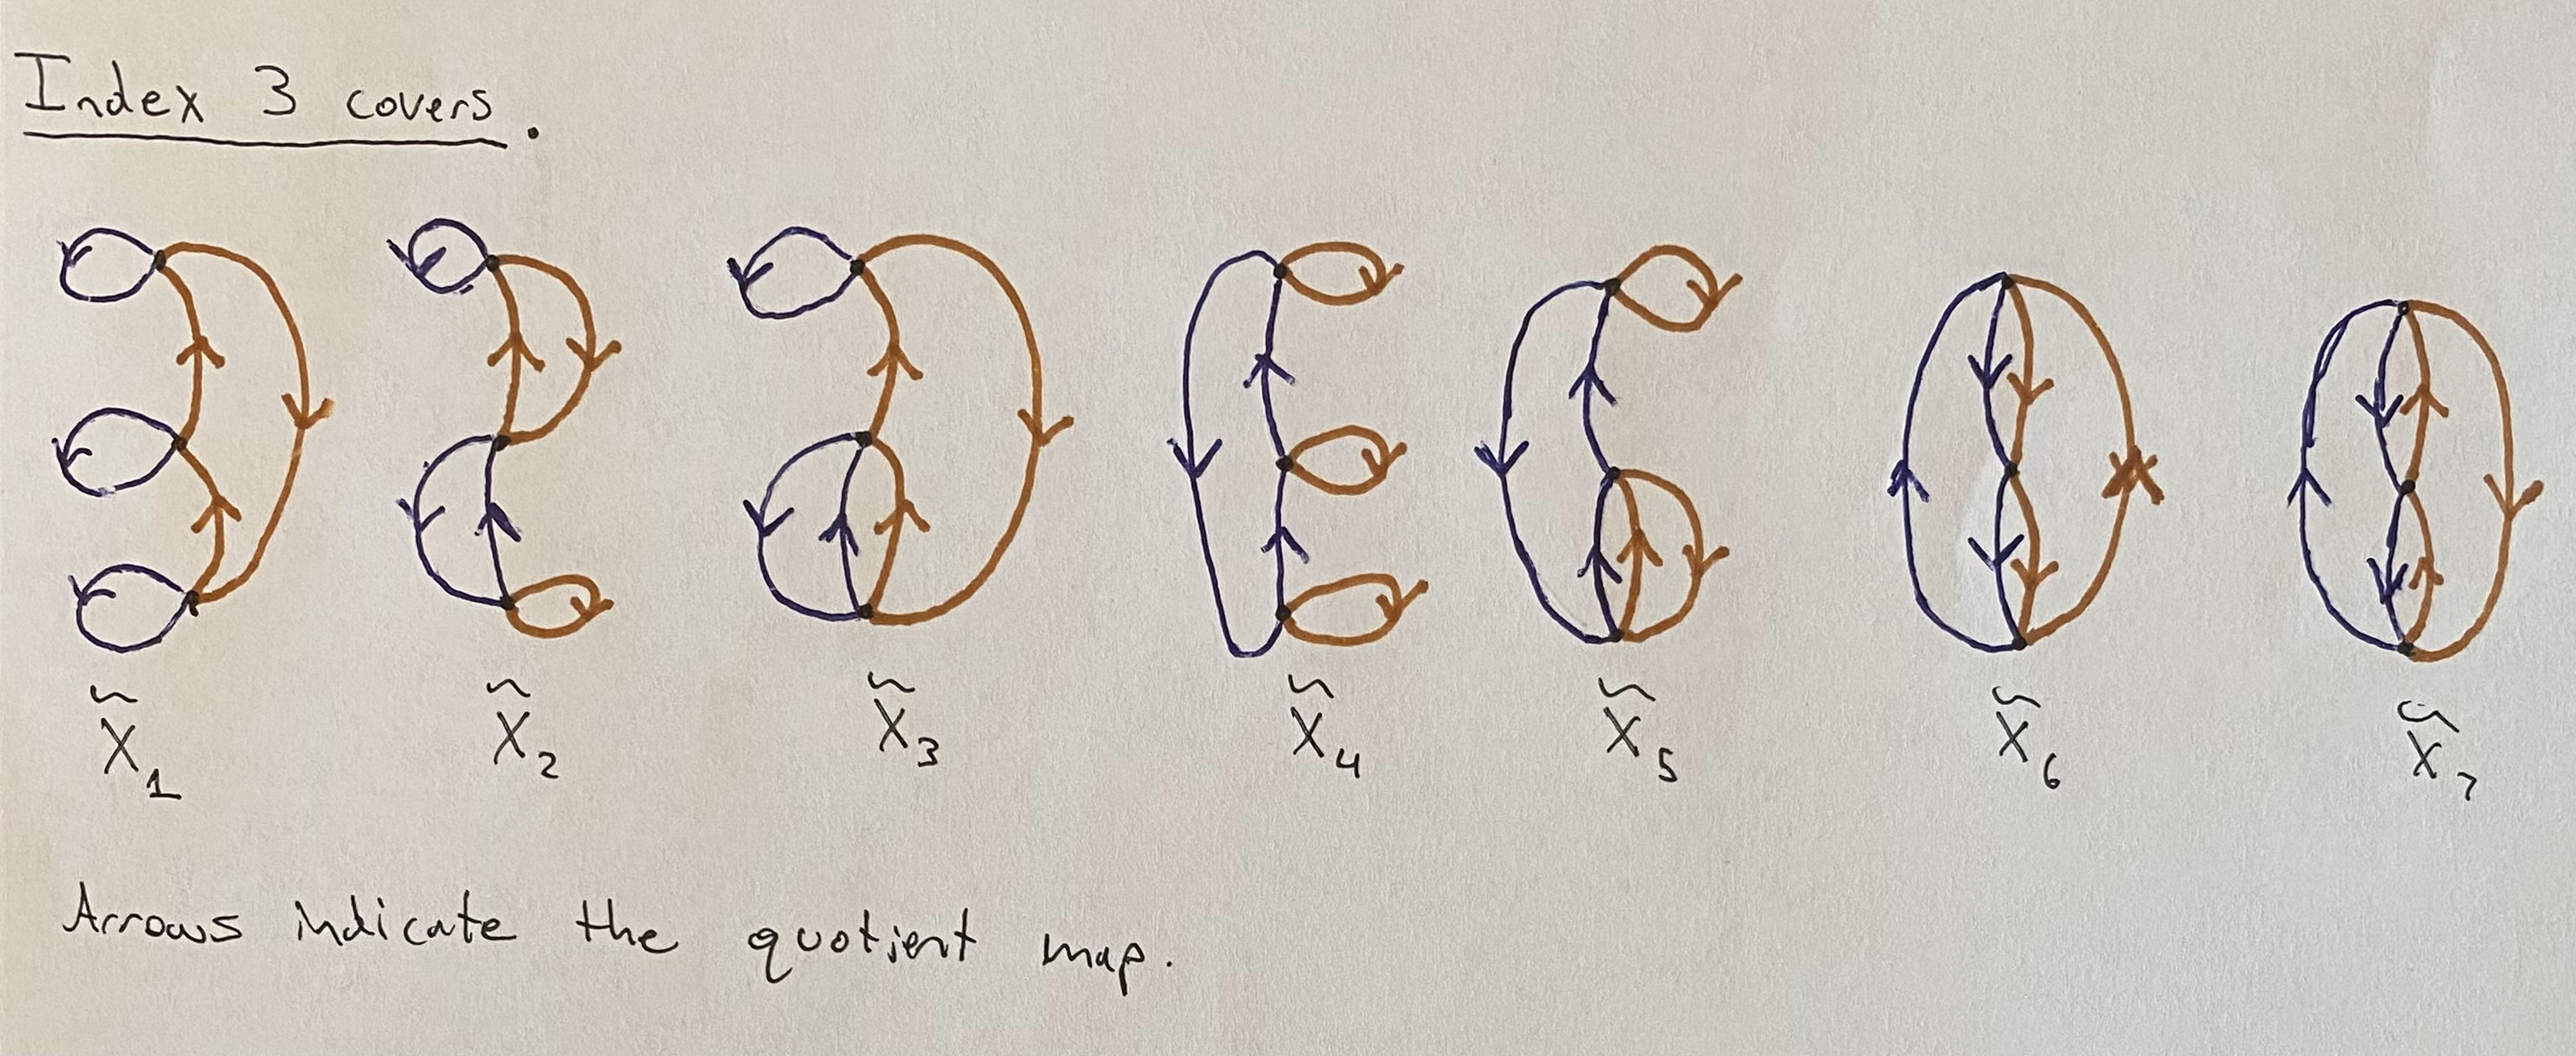
\includegraphics[width = \textwidth]{graphics/Degree 3 covers.jpg}
        \end{figure*}
        
        Because there are many more cases to consider than part (a), and the reasoning is similar I will be a bit less explicit in this section, but try to explain the reasoning for each step.

        Once again, \(x_0\) will refer to the base point of the two circles and \(G\) to \(\pi_1(X,x_0)\), with spaces as labelled in the picture use the notation \((\tilde{X_i},p^i)_{i=1}^7\), when applicable I may use the \(\tilde{x_T},\tilde{x_M},\tilde{x_B}\) to distinguish between the Top, Middle and Bottom points in \(F_{x_0}\) for a given covering space. Then each of the three points in \(F_{x_0}\) in a covering space must have an incoming and outgoing \(a\)-cycle, This uniquely defines a permutation in \(S_3\) via the action \(a\) on each point so there are 6 cases (drawing attached). Then the covering spaces must be a combination of taking the possible \(a\) and \(b\) loops.

        \begin{figure*}[h]
            \centering
            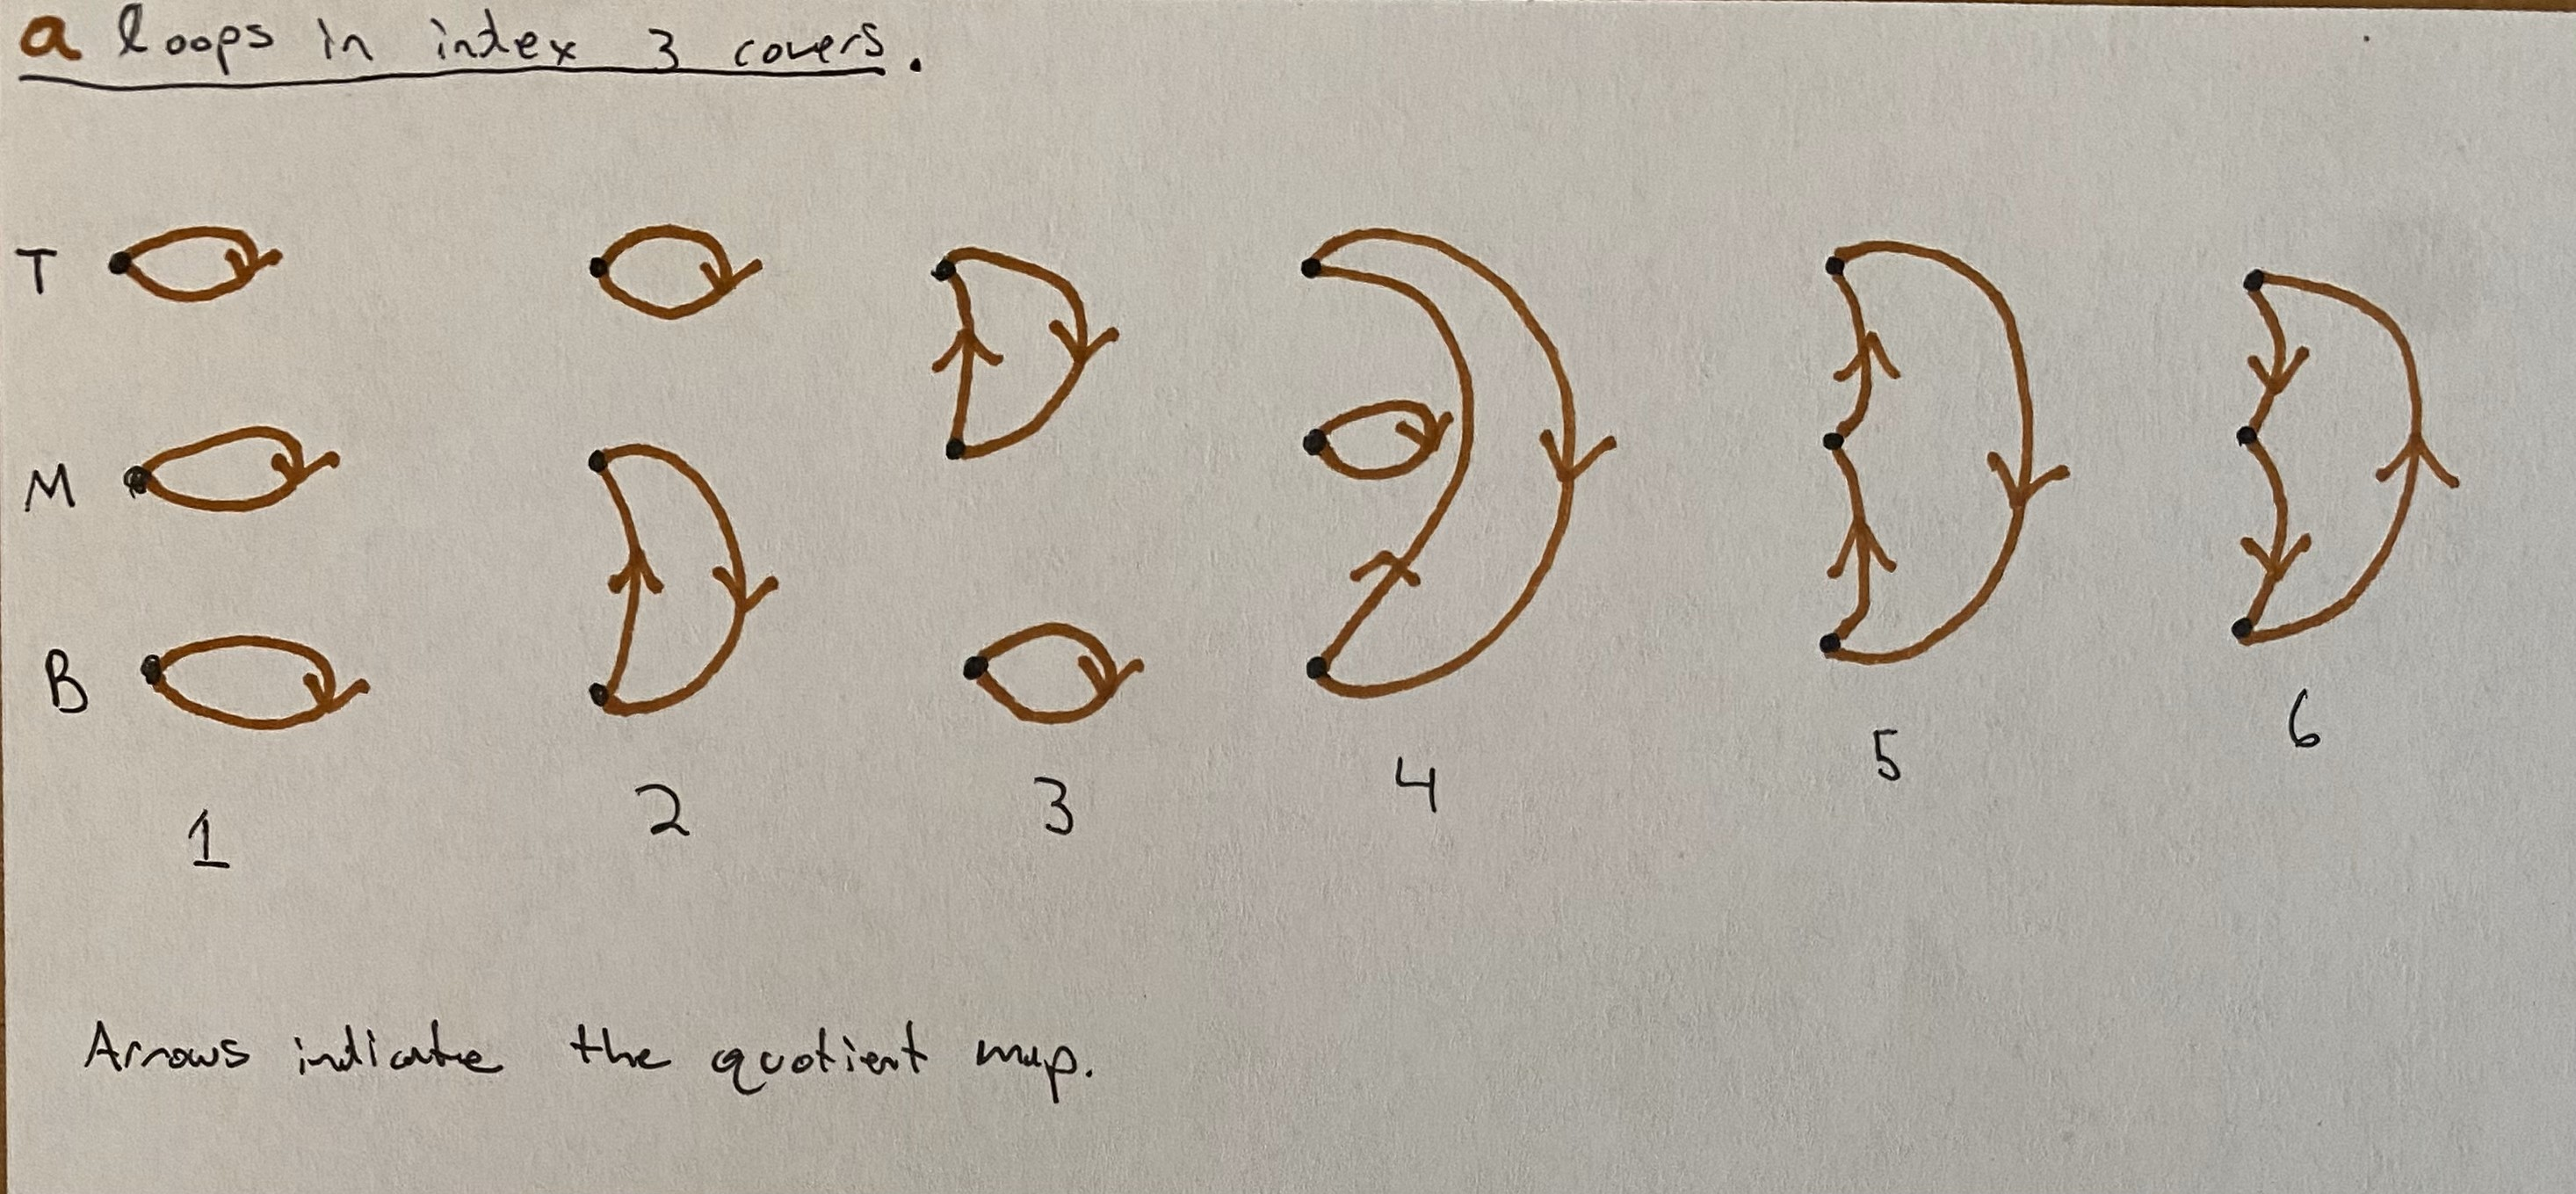
\includegraphics[width = \textwidth]{graphics/One sided loops.jpg}
        \end{figure*}

        We only consider the connected combinations, which reduces the search. Furthermore, we only need consider the sets of \(b\) loops corresponding to one sided loops 1,2 and 5 since the other loops are just permutations of these, since these are equivalent to permutations of eachother, and applying the same permutation to the \(a\) loops in a given covering space will give an isomorphic covering space for \(b\) loops 2,3 and 4 or 5 and 6.
        
        We can only pair \(b\) loops of type 1 with \(a\) loops of type 5 or 6 for connectivity, it is clear that either space of this form is isomorphic. Giving us \(\tilde{X_1}\)

        \(b\) loops of type 2 can be paired with \(a\) loops of type 3,4,5 or 6 by connectivity. It is clear that the pairings of type 3 and 4 are isomorphic, as well as pairings of type 5 and 6, which gives us \(\tilde{X_2} \tand \tilde{X_3}\)

        \(b\) loops of type 5 can be paired with any of the \(a\) loops, the covering spaces given by \(a\) loops of type 2,3,4 are isomorphic. Hence we get covering spaces of \(b\) loops with \(a\) loops of type 1,2,6 and 5. Giving us \(\tilde{X_4},\tilde{X_5},\tilde{X_6},\tilde{X_7}\).

        Before showing that these 7 covers are distinct, we first describe their Deck Transformations, since isomorphic covers will have the same group of deck transformations so this will narrow down the possibilities. Since our covering spaces have index 3, for any \(\tilde{x} \in F_{x_0}\) we have that
        \([G:p^i_*(\tilde{X_i},\tilde{x})] = 3\), and since we have multiplicativity of index, and \(G \supset N(p^i_*(\tilde{X_i},\tilde{x})) \supset p^i_*(\tilde{X_i},\tilde{x})\) we have that the normalizer sungroup is either all of \(G\) or \(p^i_*(\tilde{X_i},\tilde{x})\). So that the group of deck transformations either has cardinality 3 and \(A(\tilde{X_i},p^i) \simeq C_3\) or cardinality one and \(A(\tilde{X_i},p^i) \simeq \set{1}\) depending on these cases. One more useful fact to determine the deck transformations from the picture is that any subgroup containing the commutator is normal.

        In \(\tilde{X_1}\), fix a point \(\tilde{x_1} \in F_{x_0}\), I claim that \([G,G] \subset p^1_*(\tilde{X_1},\tilde{x_1})\). To see this, let \(\alpha \in G\), we consider its action on \(\tilde{x_1}\), a sufficient condition for \(\tilde{x_1}\cdot \alpha = \tilde{x_1}\) is when the number of \(a\) letters in \(\alpha\) is equal to the number of \(a^{-1}\) letters (I will use the fact that the multiplicity of \(a\) letters is equal to that of \(a^{-1}\) letters for elements of the commutator and similar for \(b\) and \(b^{-1}\) a lot, the proof is included at the bottom of this problem), thus the commutator subgroup fixes \(\tilde{x_1}\) which suffices to show that
        \begin{align*}
            p^1_*(\tilde{X_1},\tilde{x_1}) \lhd G \implies A(\tilde{X_1},p^1) \simeq C_3
        \end{align*}

        In \(\tilde{X_2}\), fix a point \(\tilde{x_2} \in F_{x_0}\), I claim that \(A(\tilde{X_2},p^2) = \set{1}\). To see that no non-trivial automorphism can exist, we use that one of the top or bottom points in \(F_{x_0}\) must be sent to the middle point, but \(a,b \not \in p^2_*(\pi_1(\tilde{X_2},\tilde{x_M}))\), so that the fundamental group corresponding to the top and bottom points cannot possibly be a subgroup of the middle point. Hence
        \begin{align*}
            A(\tilde{X_2},p^2) = \set{1}
        \end{align*}

        A similar argument as to \((\tilde{X_2},p^2)\) shows that there cannot be an automorphism from \(\tilde{x_T}\) to either of the middle or bottom points in the fiber since
        \begin{align*}
            b \in p^3_*(\pi_1(\tilde{X_3},\tilde{x_T})) \tand b \not \in p^3_*(\pi_1(\tilde{X_3},\tilde{x_M})) \tand b \not \in p^3_*(\pi_1(\tilde{X_3},\tilde{x_B}))
        \end{align*}
        So a non-trivial covering space morphism from \((\tilde{X_3},p^3)\) to itself cannot possibly exist since \(\tilde{x_T}\) must be sent to one of the other points in the fiber but its fundamental group is not a subset of theirs. So that
        \begin{align*}
            A(\tilde{X_3},p^3) = \set{1}
        \end{align*}
        
        The case for \((\tilde{X_4},p^4)\) is identical to that of \((\tilde{X_1},p^1)\), so we can conclude
        \begin{align*}
           A(\tilde{X_4},p^4) \simeq C_3
        \end{align*}

        \((\tilde{X_5},p^5)\) is the same case as \((\tilde{X_3},p^3)\) so we can conclude that
        \begin{align*}
            A(\tilde{X_5},p^5) = \set{1}
        \end{align*}

        Fix a point \(\tilde{x_6} \in \tilde{X_6}\), the argument for this case is similar to \((\tilde{X_1},p^1)\) in that I claim \([G,G] \subset p^6_*(\tilde{X_6},\tilde{x_6})\).
        To see this, let \(\alpha \in G\), by reading off the picture, a sufficient condition for \(\tilde{x_6}\cdot \alpha = \tilde{x_6}\) is that \(\alpha\) has as many letters \(a,b\) as it has letters \(a^{-1},b^{-1}\) this is the case for any \(\alpha \in [G,G]\). This suffices to show that
        \begin{align*}
            p^6_*(\tilde{X_6},\tilde{x_6}) \lhd G \implies A(\tilde{X_6},p^6) \simeq C_3
        \end{align*}

        Similar to the previous, fix \(\tilde{x_7} \in X_7\) then if \(\alpha \in G\) a sufficient condition for \(\tilde{x_7}\cdot \alpha\) is for \(\alpha\) to have as many letters \(a,b^{-1}\) as letters \(a^{-1},b\), this is the case for any \(\alpha \in [G,G]\) sufficing to show that
        \begin{align*}
            p^7_*(\tilde{X_7},\tilde{x_7}) \lhd G \implies A(\tilde{X_7},p^7) \simeq C_3
        \end{align*}

        All that remains to show is that the covering spaces with the same deck transformations are distinct. A useful invarient will be in a given covering space \((\tilde{X_i},p^i)\) the number of points \(\tilde{x} \in F_{x_0}\) such that \(a \in p^i_*(\pi_1(\tilde{X_i},\tilde{x}))\), as well as the same invarient for \(b\) since under any covering space morphism each of these points must be sent to a point with \(a\) (or \(b\) respectively) also in the pushforward of its fundamental group. This observation fully distinguishes \(\tilde{X_1} \tand \tilde{X_4}\) as being non-isomorphic to any of the other spaces. This also distinguishes \(\tilde{X_2}\), \(\tilde{X_3}\) and \(\tilde{X_5}\) from eachother so it only remains to show that \(\tilde{X_6} \not \simeq \tilde{X_7}\). Assume for contradiction that
        \(\phi: \tilde{X_7} \overset{\simeq}{\to} \tilde{X_6}\), then Let \(\tilde{x_7} \in F^7_{x_0} \subset \tilde{X_7}\) with image \(\tilde{x_6} \in F^6_{x_0} \subset \tilde{X_6}\).
        Then we have that
        \begin{align*}
            ab \in p^7_*\pi_1(\tilde{X_7},\tilde{x_7}) \subset p^6_*\pi_1(\tilde{X_6},\tilde{x_6})
        \end{align*}
        But from the picture, for any \(\tilde{x} \in F^6_{x_0}\) we have \(\tilde{x}\cdot ab \neq \tilde{x}\) so we have reached a contradiction.

        \textbf{Proposition.} \(\alpha \in [G,G] \implies\) The number of letters \(a\) and \(a^{-1}\) are equal in the reduced word \(\alpha\) as well as the number of letters \(b\) and \(b^{-1}\)

        Note that reduction of a word cancels equally as many \(a\) terms as \(a^{-1}\) terms, similarly for \(b\) so that a both \(N_a(\alpha) :=\) \(a\) letters \(- a^{-1}\) letters in \(\alpha\) and \(N_b(\alpha)\) = \(b\) letters \(- b^{-1}\) letters in \(\alpha\) are not affected by reduction. Furthermore, rearranging the letters of \(\alpha\) does not change \(N_a(\alpha) \tand N_b(\alpha)\). Now let \(\alpha \in [G,G]\), then \(\alpha\) can be written as \(\beta\gamma\beta^{-1}\gamma^{-1}\) (considering this in unreduced form does not change the invarients we are interested in as just described).
        But then applying the rearrangement of words preserves \(N_a\) and \(N_b\)
        \begin{align*}
            &N_a(\alpha) = N_a(\beta\gamma\beta^{-1}\gamma^{-1}) = N_a(\beta\beta^{-1}\gamma\gamma^{-1}) = N_a(1) = 0 \\
            &N_b(\alpha) = N_b(\beta\gamma\beta^{-1}\gamma^{-1}) = N_b(\beta\beta^{-1}\gamma\gamma^{-1}) = N_b(1) = 0 
        \end{align*}
    \end{pb}
    \newpage
    \begin{pb}
        In order for \(p\) to be a group homomorphism we require the following diagram commute:

        \begin{equation*} 
            \begin{tikzcd}
                (\tilde{G} \times \tilde{G},(\tilde{e},\tilde{e}))\arrow[r, "\tilde{m}"] \arrow[d, "p \times p"]& (\tilde{G},\tilde{e})\arrow[d, "p"]\\
                (G\times G, (e,e))\arrow[r, "m"]& (G,e)
            \end{tikzcd}
        \end{equation*}

        This of course implies that \(\tilde{m}\) must satisfy the lifting property described in the following diagram:

        \begin{equation*}
            \begin{tikzcd}
                &(\tilde{G},\tilde{e})\ar[d, "p"]\\
                (\tilde{G} \times \tilde{G},(\tilde{e},\tilde{e}))\ar[r, "m\circ (p \times p)"]\ar[ru, "\tilde{m}", dashed]&(G,e)
                \end{tikzcd}
        \end{equation*}

        The by the general lifting theorem, a necessary and sufficient condition for such a map to exist is
        \begin{align*}
            (m\circ(p\times p))_*\pi_1(\tilde{G}\times\tilde{G},(\tilde{e},\tilde{e})) \subset p_* \pi_1(\tilde{G},\tilde{e})
        \end{align*}

        \textbf{Uniqueness of} \(\mathbf{\tilde{m}}\) :
        in order for \(\tilde{e}\) to be the identity we require that \(\tilde{m}(\tilde{e},\tilde{e}) = \tilde{e}\), as previously stated, enforcing that \(p\) is a group homomorphism requires that \(\tilde{m}\) is a lift of \(m \circ (p \times p)\), but then since a product of connected spaces is connected, we have that any \(\tilde{m}'\) satisfying the same condition is a lift of the same map which agrees on the point \((\tilde{e},\tilde{e})\), and hence must be an identical map by connectivity of \(\tilde{G}\times \tilde{G}\).

        \textbf{The map} \(\mathbf{(m \circ (p\times p))_*}\) : By functoriality, we can write 
        \((m \circ (p\times p))_* = m_* (p\times p)_*\), so for our purposes we only need study the map \(m_*\) on \(\pi_1(G \times G,(e,e))\), we know that for any path of the form \((\alpha,1_e), \; [\alpha] \in \pi_1(G,e)\) that \(m \circ (\alpha,1_e) (t) = \alpha(t)\), so that in particular \(m_* [\alpha,1_e] = [\alpha]\) (same for paths of the form \((1_e,\alpha)\)), so we aim to use this to study \(m_*\). Denote the projection maps \(\theta_1,\theta_2: G^2 \to G\), where \(\theta_1\) projects onto the first coordinate and \(\theta_2\) the second. Then we have the isomorphism (page 77 of Massey) \(\pi_1(G \times G,(e,e)) \to \pi_1(G,e) \times \pi_1(G,e)\) given by \([\gamma] \overset{\theta}{\mapsto} ((\theta_1)_*[\gamma],(\theta_2)_*[\gamma])\). Then we have that the equivalence class of paths given by \((\theta_1\circ\gamma, e)\cdot(e,\theta_2\circ\gamma)\) maps under \(\theta\) to the same equivalence class of paths as \(\gamma\), since \(\theta\) is an isomorphism they are equal, so in particular we can write the path \([\gamma] = [\alpha,1_e][1_e,\beta]\) where \([\alpha], [\beta] \in \pi_1(G,e)\) (also note that if \([\gamma] \in p_*\pi_1(\tilde{G} \times{\tilde{G}},(\tilde{e},\tilde{e}))\), then \((\theta_i)_*[\gamma] \in p_*\pi_1(\tilde{G},\tilde{e})\), since \(\theta\vert_{p_*\pi_1(\tilde{G}\times\tilde{g},(\tilde{e},\tilde{e}))}: p_*\pi_1(\tilde{G}\times\tilde{G},(\tilde{e},\tilde{e})) \to p_*\pi_1(\tilde{G},\tilde{e}) \times p_*\pi_1(\tilde{G},\tilde{e})\)). Since \(m_*\) is a homomorphism of covering spaces, we have for \([\gamma] \in \pi_1(G\times G, (e,e)), [\gamma] = [\alpha,1_e][1_e,\beta]\) 
        \begin{align*}
            m_*([\gamma]) = m_*([\alpha,1_e][1_e,\beta]) = m_*([\alpha,1_e])m_*([1_e,\beta]) = [\alpha][\beta]
        \end{align*}

        \textbf{Existence of }\(\mathbf{\tilde{m}}\) : By our characterization of the map \((m \circ (p\times p))_*\) we have that 
        \begin{align*}
            &(m \circ (p\times p))_*\pi_1(\tilde{G}\times\tilde{G},(\tilde{e},\tilde{e})) = (p_*\pi_1(\tilde{G},\tilde{e}))(p_*\pi_1(\tilde{G},\tilde{e})) \subset p_*\pi_1(\tilde{G},\tilde{e}) \\
            &\text{where } (p_*\pi_1(\tilde{G},\tilde{e}))(p_*\pi_1(\tilde{G},\tilde{e})) := \set{[\gamma][\alpha]\;\vert \; \gamma, \alpha \in p_*\pi_1(\tilde{G},\tilde{e})}
        \end{align*}
        Hence by the lifting theorem \(\tilde{m}\) exists, we need not check for continuity since this is guaranteed by the lifting theorem.

        \textbf{Associativity of} \(\mathbf{\tilde{m}}\) : Let \(1\) denote the identity map \(G \to G\) similarly \(\tilde{1}\) on \(\tilde{G} \to \tilde{G}\). We note that by associativity of \(m\), we have the following equality of maps (\(\tilde{G}^3 \to G\)):
        \begin{align*}
            m \circ (1 \times m) \circ p^3 = m \circ (m \times 1) \circ p^3
        \end{align*}
        To show associativity of \(\tilde{m}\), we need to show that \(\tilde{m} \circ (\tilde{1} \times \tilde{m}) = \tilde{m} \circ (\tilde{m} \times \tilde{1})\), but this is simple because we only need show that the two are lifts of the two equal maps above, hence lifts of the same map, then by connectivity of \(\tilde{G}^3\) it will suffice to show they agree on a single point for equality. To see they are lifts is straightforward, since we can use the property of our first diagram commuting (i.e. \(p\) is a homomorphism wrt. \(\tilde{m}\) by construction of \(\tilde{m}\)). Furthermore we know that they agree on \(\tilde{e}^3\), by \(\tilde{m}\)'s construction as a map of pointed spaces. The computations are as follows
        \begin{align*}
            &p\tilde{m} \circ (\tilde{1} \times \tilde{m}) = m \circ (p \times p\tilde{m})
            = m \circ (p \times m\circ(p \times p)) = m \circ (1 \times m) \circ p^3 \\
            &p\tilde{m} \circ (\tilde{m} \times \tilde{1}) = m \circ(p\tilde{m}\times p) = m \circ (m \circ (p \times p),p) = m \circ (m \times 1) \circ p^3\\
            &\tilde{m} \circ (\tilde{1} \times \tilde{m})(\tilde{e}^3) = \tilde{m}(\tilde{e},\tilde{m}(\tilde{e},\tilde{e})) = \tilde{m}(\tilde{e},\tilde{e}) = \tilde{e} = \tilde{m}(\tilde{e},\tilde{e}) = \tilde{m}(\tilde{m}(\tilde{e},\tilde{e}),\tilde{e}) = \tilde{m}\circ(\tilde{m} \times \tilde{1})(\tilde{e})
        \end{align*}
        
        \(\mathbf{\tilde{e}}\) \textbf{is Identity} : The identity map \(\tilde{1}: \tilde{G} \to \tilde{G}\) exists and is a map (continuous), since \(\tilde{m}(\tilde{e},\tilde{e}) = \tilde{e} = \tilde{1}(\tilde{e})\), it suffices to check that the three maps \(p\circ\tilde{m}(\tilde{e},\tilde{1}), p\circ\tilde{1}, p\circ\tilde{m}(\tilde{1},\tilde{e})\) are all equal, hence they will all be lifts of the same map agreeing on the point \(\tilde{e}\), hence equal by connectivity of \(\tilde{G}\). But this is immediate since \(p\circ\tilde{1} = 1\circ p\), and since \(m\) is a group operation with identity \(e\), we have \(m(e,1) = m(1,e) = 1\), the following verification completes the proof of \(\tilde{e}\) being identity with respect to \(\tilde{m}\)
        \begin{align*}
            &p\circ\tilde{m}(\tilde{e},\tilde{1}) = m(p(\tilde{e}),p\circ \tilde{1}) = m(e,1)\circ p = 1 \circ p \\
            &p\circ\tilde{m}(\tilde{1},\tilde{e}) = m(p\circ \tilde{1},p(\tilde{e})) = m(1,e)\circ p = 1 \circ p
        \end{align*}

        It remains to construct the inverse map, once again we will appeal to the lifting theorem so continuity will be immediate. In order for \(p\) to be a homomorphism, we require the following diagram commute:
        \begin{equation*} 
            \begin{tikzcd}
                (\tilde{G},\tilde{e})\arrow[r, "\tilde{i}"] \arrow[d, "p"]& (\tilde{G},\tilde{e})\arrow[d, "p"]\\
                (G,e)\arrow[r, "i"]& (G,e)
            \end{tikzcd}
        \end{equation*}

        This imposes that \(\tilde{i}\) is a lift of \(i \circ p\), so we need to show there exists a map satisfying the following diagram:

        \begin{equation*}
            \begin{tikzcd}
                &(\tilde{G},\tilde{e})\ar[d, "p"]\\
                (\tilde{G},\tilde{e})\ar[r, "i \circ p"]\ar[ru, "\tilde{i}", dashed]&(G,e)
                \end{tikzcd}
        \end{equation*}

        \textbf{Existence of }\(\mathbf{\tilde{i}}\) :
        By the lifting theorem, a necessary and sufficient condition for \(\tilde{i}\) to exist is that \((i \circ p)_* \pi_1(\tilde{G},\tilde{e}) \subset p_*\pi_1(\tilde{G},\tilde{e})\), but this is immediate, since
        \[(i \circ p)_* \pi_1(\tilde{G},\tilde{e}) = i_*p_*\pi_1(\tilde{G},\tilde{e}) \subset p_*\pi_1(\tilde{G},\tilde{e})\]
        Hence by the lifting theorem the lift \(\tilde{i}\) exists.

        \textbf{Uniqueness of }\(\mathbf{\tilde{i}}\) : As discussed above, any other \(\tilde{i}'\) which is an inverse map must satisfy the property of being a lift of \(i \circ p\), for \(p\) to be a homomorphism, furthermore for \(\tilde{e}\) to be the identity, we force that \(\tilde{i}'(\tilde{e}) = \tilde{e}\), hence \(\tilde{i}\) and \(\tilde{i}'\) are lifts of the same map agreeing on a point, so by connectivity of \(\tilde{G}\) they agree on all of \(\tilde{G}\).

        \(\mathbf{\tilde{i}}\) \textbf{is an Inverse Map} : Define the following maps,
        \begin{align*}
            &\tilde{i}_R: \tilde{G} \to \tilde{G}^2, \; \tilde{i}_R: g \mapsto (g,\tilde{i}(g)) \\
            &\tilde{i}_L: \tilde{G} \to \tilde{G}^2, \; \tilde{i}_L: g \mapsto (\tilde{i}(g),g) \\
            &c_{\tilde{e}}: \tilde{G} \to \tilde{G}, \; c_{\tilde{e}}: g \mapsto \tilde{e} \\
            &c_e: G \to G, \; c_e: g \mapsto e 
        \end{align*}
        To show that \(\tilde{i}\) is an inverse map it will suffice to show that \(\tilde{m}\circ \tilde{i}_R, \tilde{m}\circ\tilde{i}_L \tand c_{\tilde{e}}\) are all lifts of the same map \(c_e\) agreeing on a point. To show this, we simply use the property from our commutative diagram for \(\tilde{i}\), namely \(p\circ\tilde{i} = i \circ p\). Note that since \(i\) is an inverse map with respect to \(m\), we have that \(m\circ(i \times 1) = m\circ(1 \times i) = c_e\)
        \begin{align*}
            &p\circ c_{\tilde{e}} = c_e \circ p \\
            &p\tilde{m}\circ \tilde{i}_R = m\circ p \tilde{i}_R = m\circ(p \times p\circ\tilde{i}) = m \circ (1 \times i) \circ p = c_e \circ p \\
            &p\tilde{m}\circ \tilde{i}_L = m\circ p \tilde{i}_L = m\circ(p\circ\tilde{i} \times p) = m \circ (i \times 1) \circ p = c_e \circ p \\
            &c_{\tilde{e}}(\tilde{e}) = \tilde{e} \\
            &\tilde{m}\circ\tilde{i}_R(\tilde{e}) = \tilde{m}(\tilde{e},\tilde{i}(\tilde{e})) = \tilde{m}(\tilde{e},\tilde{e}) = \tilde{e} \\
            &\tilde{m}\circ\tilde{i}_L(\tilde{e}) = \tilde{m}(\tilde{i}(\tilde{e}),\tilde{e}) = \tilde{m}(\tilde{e},\tilde{e}) = \tilde{e}
        \end{align*}
        So that by connectedness of \(\tilde{G}\) the three maps are equal since they are lifts of the same map and agree at a point.

        This concludes the proof of existence and uniqueness of a topological group structure on \(\tilde{G}\), with identity \(\tilde{e}\) and such that \(p: \tilde{G} \to G\) is a homomorphism. Note that \(p\) satisfies the homomorphism properties by construction of \(\tilde{m} \tand \tilde{i}\) and that they are also continuous by construction.
        
    \end{pb}
    \newpage
    \begin{pb}
        Once again let \(x_0\) denote the base point of the two circles \(S^1 \vee S^1\). We denote \(G:= \pi_1(X,x_0) = \gen{a}*\gen{b}\).

        The covering space is given by \(\tilde{X} = \mathbb{R} \times \mathbb{Z} \cup \mathbb{Z} \times \mathbb{R}\) with the subspace topology on \(\mathbb{R}\). Consider the action of \(\mathbb{Z}^2\) on \(\tilde{X}\) where for \((x,y) \in \tilde{X}\) we take \((x,y) \cdot(n,m) = (x+n,y+m)\) this action is clearly free since \((x,y) = (x+n,y+m) \iff (n,m) = (0,0)\). This action is also properly discontinuous since under the induced topology from \(\mathbb{R}^2\) if \((n,m) \neq (0,0) \in \mathbb{Z}^2\)
        \begin{align*}
            d\left((x,y), (x+n,y+m) \right) = \sqrt{n^2 + m^2} \geq 1
        \end{align*}
        and since \(\mathbb{Z}^2\) acts on open sets via translation it will suffice to choose a neighborhood of radius \(< \frac12\) for the properly discontinuous condition to hold. (i.e. \(U \cap (U\cdot g) = \emptyset, \; \forall g \in \mathbb{Z}^2\)).

        It follows from our converse theorem from class that \((\tilde{X},p)\) (where \(p\) is the quotient map) is a normal covering space for \(\tilde{X}/\mathbb{Z}^2 \cong X\) (this should be sufficiently clear from the construction but also see picture) with group of deck transformations \(A(\tilde{X},p) \simeq \mathbb{Z}^2\) acting via translation on the grid.

        \begin{figure*}[h]
            \centering
            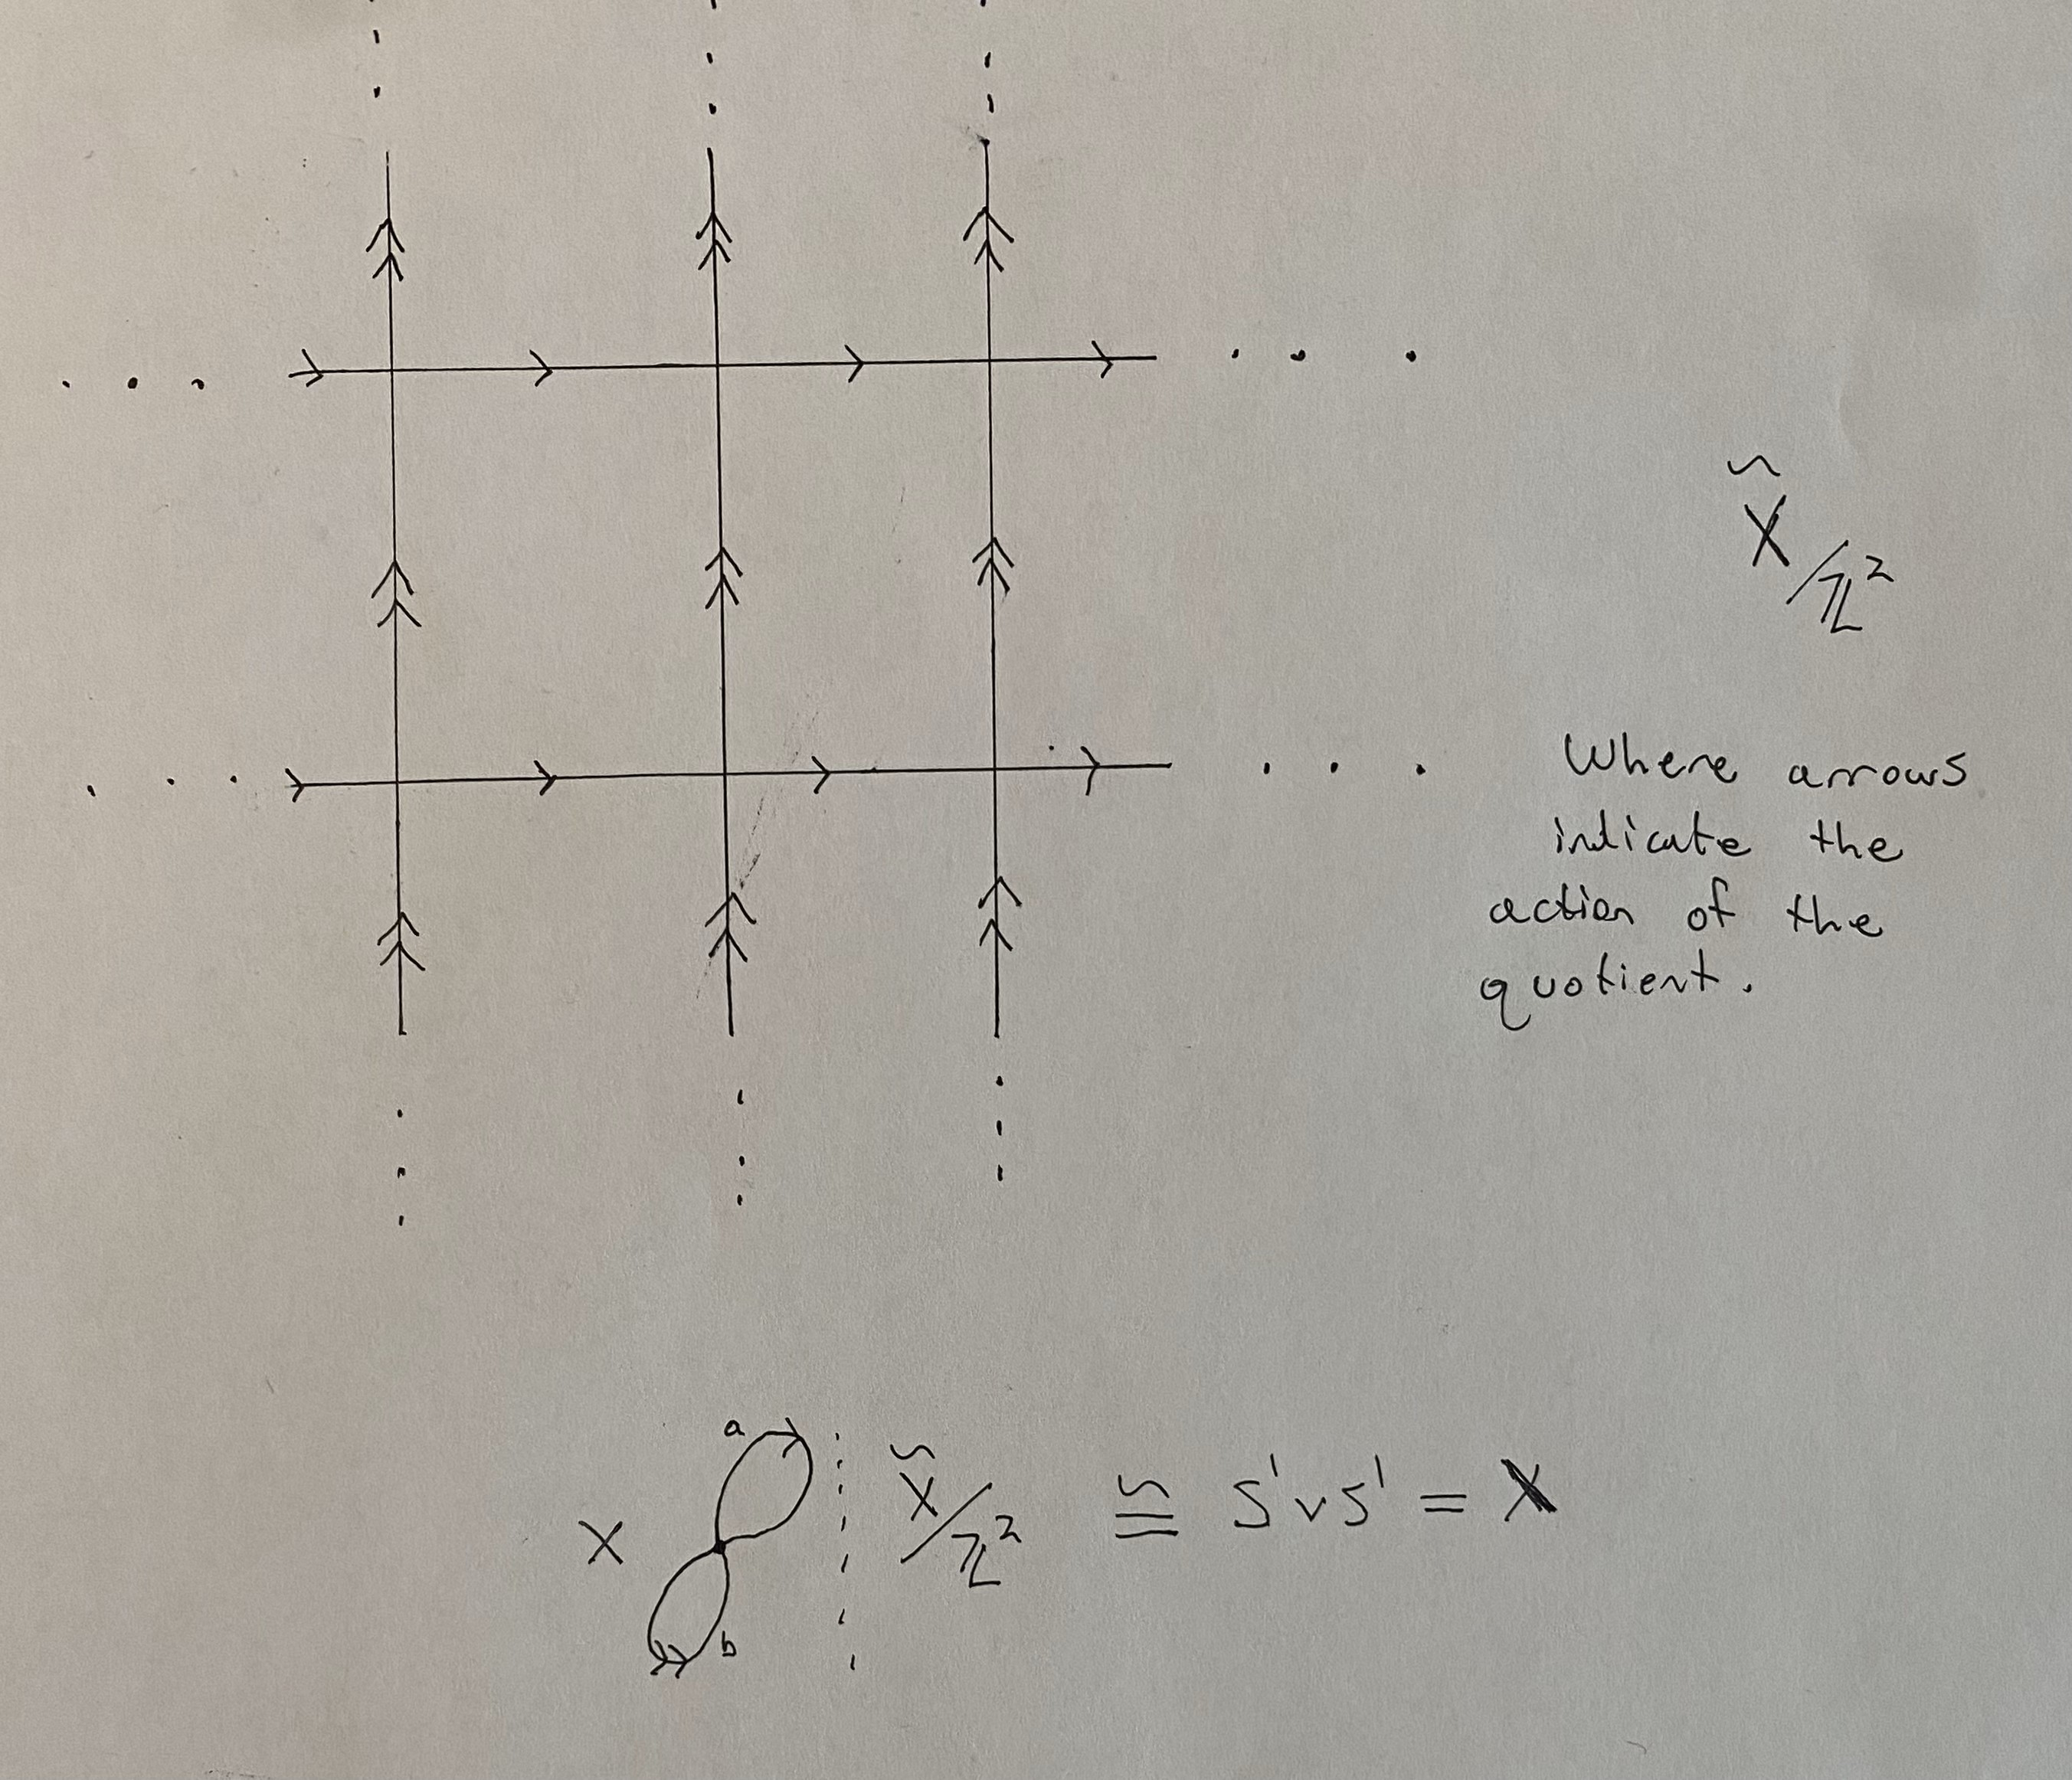
\includegraphics[width = \textwidth]{graphics/Covering space grid.jpg}
        \end{figure*}

        To conclude that \(\tilde{X}\) corresponds to \([G,G]\), we let \(\tilde{x_0} \in F_{x_0}\)
        we first note that since \(p_*\pi_1(\tilde{X},\tilde{x_0})\) is normal in \(\pi_1(X,x_0)\) (since \(\tilde{X}\) is a normal covering space) \(A(\tilde{X},p) = \frac{\pi_1(X,x_0)}{p_*\pi_1(\tilde{X},\tilde{x_0})} \simeq \mathbb{Z}^2\) is abelian, and hence \([\pi_1(X,x_0),\pi_1(X,x_0)] \subset p_*\pi_1(\tilde{X},\tilde{x_0})\). We only need to prove the other set inclusion. Consider the natural inclusions \(\tilde{X} \overset{\tilde{\iota}}{\to} \mathbb{R}^2\), and \(X \overset{\iota}{\to} T^2\), it is clear that the following diagram commutes, where \(p'\) is the map making \(\mathbb{R}^2\) the universal covering space of \(T^2\):

        \begin{equation*} 
            \begin{tikzcd}
                (\tilde{X},\tilde{x_0})\arrow[r, "\tilde{\iota}"] \arrow[d, "p"]& (\mathbb{R}^2,\tilde{x_0})\arrow[d, "p'"]\\
                (X,x_0)\arrow[r, "\iota"]& (T^2,x_0)
            \end{tikzcd}
        \end{equation*}

        Furthermore, we have \(\iota_*\pi_1(X,x_0) = \pi_1(T^2,x_0) = \gen{a} \times \gen{b} = \pi_1(X,x_0)_{\text{Abelian}}\), so that the kernel of this map is exactly \newline \([\pi_1(X,x_0),\pi_1(X,x_0)]\)
        Applying the \(\pi_1\) functor to the diagram gives us that
        \begin{align*}
            (\iota \circ p)_*\pi_1(\tilde{X},\tilde{x_0}) = (p'\circ \tilde{\iota})\pi_1(\tilde{X},\tilde{x_0}) \subset p'_* (\mathbb{R}^2,\tilde{x_0}) = \set{1}
        \end{align*}
        By functoriality, we have that \( (\iota \circ p)_*\pi_1(\tilde{X},\tilde{x_0}) = \iota_* p_* \pi_1(\tilde{X},\tilde{x_0})\), which allows us to conclude that
        \begin{align*}
            p_*\pi_1(\tilde{X},\tilde{x_0}) \subset \ker \iota_* = [\pi_1(X,x_0),\pi_1(X,x_0)]
        \end{align*}
        So that with both set inclusions \(p_*\pi_1(\tilde{X},\tilde{x_0}) = [\pi_1(X,x_0),\pi_1(X,x_0)]\) proving that this is indeed the covering space corresponding to the commutator subgroup.

        As previously mentioned the group of deck transformations is isomorphic to \(\mathbb{Z}^2\). with action \((x,y)\cdot (n,m) = (x+n,y+m)\) by construction so that the deck transformations act by translating the infinite grid.

    \end{pb}
\end{document}